\chapter{The Search for the Supersymmetric Top-quark}
\label{chap:search_stop}

\epigraph{
\textit{It will be remembered that the 18$^{th}$ century was, on the whole,
addicted to an ascending series of living forms shading by insensible degrees
into each other and leading onto man.
There was no consideration of the fact that this might be reading into Nature a greater
unity than she actually possessed. It led inevitably to some highly
questionable taxonomy produced in the effort to compress all life into positions upon a
single stairway.}
}
{
--Loren Eiseley, \textit{Darwin's Century}
}

\epigraph{
\textit{Cease, cows, life is short.}
}
{
--Gabriel Garc\'{i}a M\'{a}rquez, \textit{One Hundred Years of Solitude}
}

%%%%%%%%%%%%%%%%%%%%%%%%%%%%%%%%%%%%%%%%%%%%%%%%%%%%%%%%%%%%%%%%%%%%%%%%%%%%%%%%%%%%%%%%
%%%%%%%%%%%%%%%%%%%%%%%%%%%%%%%%%%%%%%%%%%%%%%%%%%%%%%%%%%%%%%%%%%%%%%%%%%%%%%%%%%%%%%%%
%%%%%%%%%%%%%%%%%%%%%%%%%%%%%%%%%%%%%%%%%%%%%%%%%%%%%%%%%%%%%%%%%%%%%%%%%%%%%%%%%%%%%%%%
%%%%%%%%%%%%%%%%%%%%%%%%%%%%%%%%%%%%%%%%%%%%%%%%%%%%%%%%%%%%%%%%%%%%%%%%%%%%%%%%%%%%%%%%

As described in Chapter~\ref{chap:bsm}, the lighter mass eigenstate of the superpartner of
the top quark, $\stopone$, plays an important role in helping solve the Hierarchy problem.
Most SUSY scenarios prefer \stopone masses not much larger than $1\,\TeV$, so as to keep them
at the scale EWSB.
If the \stopone exists, and is indeed lighter than the \TeV~scale, it may easily be produced in the $13\,\TeV$ $pp$ collisions
occurring at the LHC.
Searches for stops therefore play a prominent role in the searches for SUSY in ATLAS.

This chapter presents a search for the production of stop quarks.
The SUSY model considered here satisfies $R$-parity conservation, as do the majority of SUSY
searches at the LHC, which forces the \stopone to be produced in pairs and to follow
a decay chain ending in the stable LSP.
The LSP in these models is assumed to be the lightest neutralino, \ninoone.

SUSY searches performed in ATLAS are done using so-called `simplified models', wherein all parameters
of the MSSM are selected except for the masses of the sparticles relevant to the decays
of the sparticle being searched for.
For the case presented in this chapter, a search for \stopone is described and the simplified models
used to describe the SUSY signal process are parametrised by two free parameters: the mass of the 
\stopone and the mass of the \ninoone.
With these two parameters defined, the kinematics and production cross-section are fixed.
In the models considered, the \stopone is classified into three regions of phase space according
to the mass of the \ninoone, into which it decays.
The potential decays of the \stopone are illustrated by the decay diagrams in Figure~\ref{fig:stop_diagrams}.
showing the cases of the two-, three-, and four-body decays of the \stopone.
These decays are associated with three different regions of parameter space in the $(m_{\stopone}, m_{\ninoone})$ plane,
illustrated in Figure~\ref{fig:stop_boundaries}.
The analysis to be discussed in this chapter reports the results of a search for the production
of \stopone particles following the three-body decay, in which the mass-difference between the \stopone
and \ninoone, \sdiff, is less than (greater than) the mass of the SM top-quark ($W+b$ system).
This is the middle region of phase space indicated in Figure~\ref{fig:stop_boundaries}, $\stopone \rightarrow b W \ninoone$.
In this region, the two-body \stopone decays are kinematically suppressed and the \stopone decays via
an off-shell top-quark or \chinoonepm to the three-body $b W \ninoone$ final state.

\begin{figure}[!htb]
    \begin{center}
        \includegraphics[width=0.3\textwidth]{figures/search_stop2l/signal/fgraph_stop_tN} \hspace{1cm}
        \includegraphics[width=0.3\textwidth]{figures/search_stop2l/signal/fgraph_stop_bCN} \\
        \includegraphics[width=0.3\textwidth]{figures/search_stop2l/signal/fgraph_3body} \hspace{1cm}
        \includegraphics[width=0.3\textwidth]{figures/search_stop2l/signal/fgraph_stop_bffN}
        \caption{
            Decay diagrams for the \stopone relevant to the two-lepton final state of \stopone pair-production.
            \textit{\textbf{Top}}: Diagrams leading to the two-body decay of the \stopone, either
                into $\stopone \rightarrow t \ninoone$ (\textit{top left}) or $\stopone \rightarrow b \chinoonepm$ (\textit{top right}).
            \textit{\textbf{Bottom left}}: Three-body decay of the \stopone, $\stopone \rightarrow b W \ninoone$.
            \textit{\textbf{Bottom right}}: Four-body decay of the \stopone, $\stopone \rightarrow b f f^{\prime} \ninoone$.
        }
        \label{fig:stop_diagrams}
    \end{center}
\end{figure}

\begin{figure}[!htb]
    \begin{center}
        \includegraphics[width=0.7\textwidth]{figures/search_stop2l/signal/stop_LSP_boundaries}
        \caption{
            Kinematic boundaries in the (\stopone,\ninoone) plane, indicating the three kinematic
            regimes associated with the decay of the \stopone: the two-body $\stopone \rightarrow t \ninoone$
            decay ($\Delta m(\stopone, \ninoone) > m_t$), the three-body $\stopone \rightarrow b W \ninoone$ decay
            ($\Delta m(\stopone, \ninoone) < m_t$), and the four-body $\stopone \rightarrow b f f^{\prime} \ninoone$
            decay ($\Delta m(\stopone, \ninoone) < m_b + m_W$).
            Here $\Delta m(\stopone, \ninoone) = m_{\stopone} - m_{\ninoone}$.
        }
        \label{fig:stop_boundaries}
    \end{center}
\end{figure}

Figure~\ref{fig:run1_stop_summary} shows the results of the searches for \stopone particles performed
in Run 1 of the LHC by the ATLAS experiment.
This figure indicates the regions of SUSY parameter space, under the hypothesis of the
simplified model parametrised by the masses of the \stopone and \ninoone particles,
that are excluded at 95\% CL by the zero, one, and two lepton analyses.
It can be seen that the Run 1 analyses targeting the two-lepton final states did not effectively
cover the three-body regime, at least in comparison to all analyses in the two-body and four-body regions
of the $(m_{\stopone}, m_{\ninoone})$-plane.

Section~\ref{sec:susy_exclusion_plots} provides a brief introduction to the type of plots
shown in Figure~\ref{fig:run1_stop_summary}, which are the general SUSY exclusion plots
that are presented to summarise the results of SUSY searches based on simplified models
by both the ATLAS and CMS experiments.
Section~\ref{sec:stop_pheno} then begins by describing the kinematics and phenomenology of the three-body \stopone
decays that are being targeted in the SUSY analysis presented in this chapter.
With the signal kinematics in mind, Section~\ref{sec:stop_event_sel} describes the overall event
selection and object definition used in the analysis, so that the analysis' event sample can be understood.
Section~\ref{sec:stop_strategy} describes how the phenomenology described in Section~\ref{sec:stop_pheno}
motivates a particular choice of discriminating observables that are sensitive to the three-body decay
of the \stopone particle, as well as the definition of the analysis' SRs.
Section~\ref{sec:stop_background_estimate} describes the analysis' background estimation
strategy, particular the definition of CRs and VRs used to constrain the dominant
SM backgrounds.
Section~\ref{sec:stop_results} closes the chapter with the results of the search for
the three-body \stopone in the two-lepton final state.


\begin{figure}[!htb]
    \begin{center}
        \includegraphics[width=0.7\textwidth]{figures/search_stop2l/run1_stop_summary}
        \caption{
            Summary of SUSY \stopone searches in the (\stopone, \ninoone) plane
            at the end of Run 1.
            The searches relevant to the work in the present thesis are indicated by the 
            coverage of purple and dark orange: `t1L,t2L' and `WW', respectively.
            Figure taken from Ref.~\cite{StopRun1Summary}.
        }
        \label{fig:run1_stop_summary}
    \end{center}
\end{figure}

\FloatBarrier
\section{Aside: SUSY Exclusion Plots}
\label{sec:susy_exclusion_plots}

In this section we describe the typical SUSY exclusion plot, illustrated in Figure~\ref{fig:susy_exclusion_cartoon}.
These plots are used when presenting the results of SUSY searches based on the assumptions
made in simplified models of the MSSM, parametrised only by the masses of the
pair-produced sparticle and the stable sparticle appearing in the final state (the LSP), assuming $R$-parity
conservation. The main things to observe in this plot are as follows:

\begin{enumerate}
    \item The region contained \textit{within} the contours is the region of SUSY parameter space,
        under the assumption of the simplified model, excluded at 95\% CL
    \item The region in which the mass of the produced
        sparticle is less than the mass of the LSP is kinematically forbidden
    \item The analysis sensitivity (i.e. power to exclude) decreases as the mass of the produced sparticle increases
    \item The analysis sensitivity (i.e. power to exclude) decreases as $\sdiff \rightarrow 0$ ($\sdiff \rightarrow m_X$,
        with $m_X$ a mass scale related to an intermediate state appearing in the sparticle decay)
    \item The expected 95\% CL exclusion limits are reported with their $\pm 1 \sigma$ uncertainty band,
        related to the precision of the analyses based on their systematic uncertainty evaluation
    \item The observed 95\% CL exclusion limit is not reported with an error
\end{enumerate}

Item (3) in the above is related to the fact that the cross-section of the SUSY sparticle production cross-section
is a function of only the mass of the pair-produced sparticle in the simplified models assumed here.
The production cross-section decreases in proportion to the mass of the sparticle, indicated in Figure~\ref{fig:susy_xsec},
which leads to analyses becoming less sensitive to the scenarios with larger masses of the produced sparticles.

Item (4) is also relatively straightforward.
As the masses of the produced sparticle and final-state LSP become nearer to one another, and even
degenerate, kinematic phase space suppression results in there being less energy-momentum available to be transferred to the final state
particles.
This results in final state particles having typically lower energies and momenta,
making them difficult to trigger on and reconstruct efficiently.
This inefficiency reduces an analysis' sensitivity to these kinematic regimes, since the final states become experimentally
inaccessible.
This scenario also appears when the produced sparticle follows a more complex decay chain,
as in the cases illustrated in Figure~\ref{fig:stop_diagrams}, where intermediate mass scales such as the
mass of the SM top-quark or $W$-boson are introduced.
Near these regions, the kinematics of the particles decaying from the objects defining these intermediate
mass scales change rapidly.
As a result, analyses targeting particle kinematics on one side of such a boundary
cannot simultaneously be sensitive to the particle kinematics on the opposing side of the boundary.
For this reason, it is common practice to define separate analyses targeting each side of a given boundary,
as indicated in Figure~\ref{fig:run1_stop_summary}.

The expected limits in Item (5) in the above are related to running the analysis' hypothesis tests
on the SUSY scenarios indicated by the position on the $(m_{\stopone}, m_{\ninoone})$-plane,
and using for $\bm{N^{\text{obs}}}$ (c.f. Equations~\ref{eq:likelihood_main} and \ref{eq:full_likelihood}) the value in the SRs for the predicted background; that is, the
observed data counts in the analysis' signal regions are substituted with the value of the total predicted
background in the signal regions.
The observed data is still used in the CRs, which provide the normalisation correction factors as described in Section~\ref{sec:likelihood}.
The observed limits discussed in Item (6), on the other hand, take as $\bm{N^{\text{obs}}}$ the actual observed data counts
in the analysis' SRs.
Due to statistical fluctuations in the observed data, the expected and observed 95\%CL exclusion contours
do not typically overlap perfectly.

\begin{figure}[!htb]
    \begin{center}
        \includegraphics[width=0.8\textwidth]{figures/search_stop2l/susy_exclusion_cartoonPDF}
        \caption{
            Cartoon illustrating an example of a typical two-dimensional exclusion plot
            for a SUSY simplified model.
            The mass of the pair-produced SUSY particle is on the $x$-axis and the mass of the
            LSP to which it decays is on the $y$-axis.
            The region bounded by (i.e. inside of) the dashed-black (red) curves indicate
            the expected (observed) region of SUSY parameter space excluded at the 95\% CL.
            The $\pm 1\sigma$ error band is shown on the expected limits, and is based on the
            systematic uncertainties included in the analysis.
            SUSY exclusion curves such as these usually exhibit a triangular shape as a result
            of two competing effects, indicated by the arrows: 1) the reduction in production
            cross-section as the mass of the produced SUSY particle increases, and 2) kinematic
            suppression occurring when the phase space available to the final state decreases
            as a result of $\Delta m (x, y) = m_x - m_y \rightarrow 0$.
            Kinematic suppression results in the final state objects, such as leptons and $b$-tagged jets
            in the case presented in the current thesis,
            having very little momenta, thereby making it difficult to efficiently identify
            the event as being consistent with the given SUSY hypothesis being searched for.
        }
        \label{fig:susy_exclusion_cartoon}
    \end{center}
\end{figure}

\begin{figure}[!htb]
    \begin{center}
        \includegraphics[width=0.65\textwidth]{figures/search_stop2l/SUSY_xsec_13TeV_v1}
        \caption{
            Production cross-section for the SUSY sparticles indicated in the legend,
            as a function of their mass, computed as in Ref.~\cite{SUSYXsec1}.
            The bands indicate the uncertainty due to the theoretical prediction of the production
            process.
            The green band indicates the \stopone production cross-section, relevant to the analysis
            described in the current chapter.
            For comparison, the production cross-section for SM top-quark pair-production is $\approx 830$\,pb at 13\,\TeV.
        }
        \label{fig:susy_xsec}
    \end{center}
\end{figure}

\FloatBarrier
%%%%%%%%%%%%%%%%%%%%%%%%%%%%%%%%%%%%%%%%%%%%%%%%%%%%%%%%%%%%%%%%%%%%%%%%%%%
%%%%%%%%%%%%%%%%%%%%%%%%%%%%%%%%%%%%%%%%%%%%%%%%%%%%%%%%%%%%%%%%%%%%%%%%%%%
%%%%%%%%%%%%%%%%%%%%%%%%%%%%%%%%%%%%%%%%%%%%%%%%%%%%%%%%%%%%%%%%%%%%%%%%%%%
%
% SIGNAL DESCRIPTION
%
%%%%%%%%%%%%%%%%%%%%%%%%%%%%%%%%%%%%%%%%%%%%%%%%%%%%%%%%%%%%%%%%%%%%%%%%%%%
%%%%%%%%%%%%%%%%%%%%%%%%%%%%%%%%%%%%%%%%%%%%%%%%%%%%%%%%%%%%%%%%%%%%%%%%%%%
%%%%%%%%%%%%%%%%%%%%%%%%%%%%%%%%%%%%%%%%%%%%%%%%%%%%%%%%%%%%%%%%%%%%%%%%%%%
\section{Phenomenology of the Signal}
\label{sec:stop_pheno}

\section{Event Selection and Object Definition}
\label{sec:event_sel}

\section{Signal Selection Strategy}
\label{sec:hh_strategy}

%%%%%%%%%%%%%%%%%%%%%%%%%%%%%%%%%%%%%%%%%%%%%%%%%%%%%%%%%%%%%%%%%%%%%%%%%%%%%%%%%%%
%%%%%%%%%%%%%%%%%%%%%%%%%%%%%%%%%%%%%%%%%%%%%%%%%%%%%%%%%%%%%%%%%%%%%%%%%%%%%%%%%%%
%%%%%%%%%%%%%%%%%%%%%%%%%%%%%%%%%%%%%%%%%%%%%%%%%%%%%%%%%%%%%%%%%%%%%%%%%%%%%%%%%%%
%
% NN 
%
%%%%%%%%%%%%%%%%%%%%%%%%%%%%%%%%%%%%%%%%%%%%%%%%%%%%%%%%%%%%%%%%%%%%%%%%%%%%%%%%%%%
%%%%%%%%%%%%%%%%%%%%%%%%%%%%%%%%%%%%%%%%%%%%%%%%%%%%%%%%%%%%%%%%%%%%%%%%%%%%%%%%%%%
%%%%%%%%%%%%%%%%%%%%%%%%%%%%%%%%%%%%%%%%%%%%%%%%%%%%%%%%%%%%%%%%%%%%%%%%%%%%%%%%%%%


The current analysis makes use of a multi-output classifier, one that does not simply classifry
a single process against a single background label, but rather a classifier that provides multiple
output labels with each pertaining to a distinct class or process.
One of the easiest ways to build such a classifier is to take a multi-variate approach that
is by default suitable for multi-output classification: neural networks.

\subsection{Neural Network Architecture}
\label{sec:nn_arch}

The analysis makes use of a deep-learning, neural network based approach.
The classifiers that we build are trained to classify $pp$ collision events according to
four potential class labels, inspired by the dominant expected background processes:
\begin{enumerate}
    \item Dilepton non-resonant $hh \rightarrow \bbww$
    \item SM top-quark processes ($\ttbar + Wt$), `Top'
    \item SM $Z$+jets processes, $Z \rightarrow \{ee,\mu\mu\}$
    \item SM $Z$+jets processes, $Z \rightarrow \tau\tau$
\end{enumerate}
The classifier is trained with separate labels for the $Z \rightarrow \{ee,\mu\mu\}$ and
$Z \rightarrow \tau\tau$ processes as these lead to clearly different final state kinematics.
The dilepton final state that we eventually select in the analysis is composed only of electrons and muons.
The $Z \rightarrow \tau\tau$ process contributes only in the cases where both $\tau$ leptons decay
leptonically.
The electrons and muons from these $\tau$ decays have very different kinematic signatures as compared
to those from the direct decays of the $Z$-bosons.
Allowing the classifier to learn to distinguish between these $Z$ decays improves its overall performance
to separate the $hh$ signal process from the backgrounds.

%The dominant SM top-quark backgrounds, \ttbar~and single-top $Wt$ are combined into a single
%process during the training of the classifier since these two top-quark processes are found
%to have similar enough kinematics in the regions of high signal purity that separating them
%at the point of training has little effect.
%Additionally, in regions where there is large contributions from both SM \ttbar~and single-top $Wt$
%processes, particularly in the $WWbb$ final state, the two processes have non-trivial quantum
%interferene and it becomes difficult to define them separately.
%For this reason, we consider the sum of these two processes as a single background.

We construct the neural network architecture using the \textsc{Keras}~\cite{chollet2015keras}
library, using \textsc{Tensorflow}~\cite{tensorflow2015} as a backend.
An illustration of the neural network architecture is given in Figure~\ref{fig:nn_arch}.
The network inputs are passed through a dense (fully-connected) layer,  which
is trained with a dropout layer, and then a second dense layer.
The final activation is a softmax activation.

\begin{figure}[!htb]
    \begin{center}
        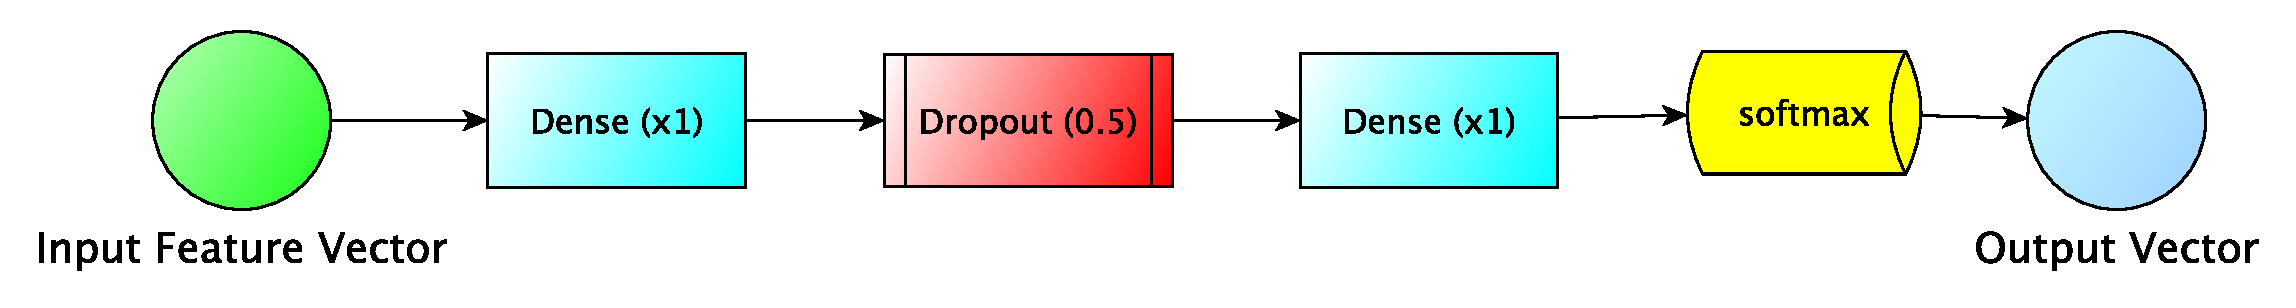
\includegraphics[width=0.85\textwidth]{figures/search_hh/mva/nn_arch_graph_updated}
        \caption{
            Illustration of the neural network graph employed in the analysis.
            The input feature vector has a length of 35 and the output vector is length 4,
            one for each of the targetted processes.
        }
        \label{fig:nn_arch}
    \end{center}
\end{figure}
Each of the dense layers are 250 nodes wide and  have their weights randomly initialized by sampling
from a truncated normal distribution centered on zero with a width given by $\sqrt{1/N_{\text{inputs}}}$, where
$N_{\text{inputs}}$ is the number of input features (the length of the input vector).
The activation functions for each of the dense layers are rectified linear units (`ReLu')~\cite{ReLu}.

Using an output layer with a softmax activation function allows one to interpret the outputs as
each representing a probability\footnote{The use of the term `probability' here is only
loosely correct, as the outputs are not \textit{strictly} probabilities.}
for the output's associated class ($hh$, Top, $Z \rightarrow \{ee,\mu\mu\}$,
or $Z \rightarrow \tau\tau$) given the inputs and for this reason it is commonly used for multi-class
neural network classifiers.
The association of the softmax activation with a class probability can be seen by its definition,
\begin{align}
    a_j = \frac{ e^{z_j} } { \sum\limits_k e ^{z_k} },
    \label{eq:softmax_activation}
\end{align}
where $a_j$ is the activation of the $j^{th}$ output neuron, the $z_i$ are the inputs to the output layer,
and $k$ runs over all output neurons.
It can be seen that if one sums over all outputs of a layer whose activation is given by Equation~\ref{eq:softmax_activation}
that the sum is equal to one.
Thus, the outputs of the softmax layer can be seen as a probability distribution.
For this reason, in the discussion to follow, we refer to the outputs of our neural network as `$p_i$',
where $i$ has four possibiities for each of the four outputs: $i \in \{ hh, \text{Top}, Z\rightarrow ee/\mu\mu, Z\rightarrow \tau\tau \}$.

The use of droput layers during the training process of is a form of statistical learning regularization that is reminiscient
of ensemble methods in the non-deep-learning arena, such as random forests~\cite{RandomForestsBreiman2001}.
They act to randomly disable a tunable fraction of inputs during various points in the training stage~\cite{JMLRDropout}.
This tunable fraction is referred to as the \textit{dropout rate}.
The use of dropout regularization prevents nodes within the network from co-adapting too much, thus reducing
the effects of overtraining.
This is illustrated in Figure~\ref{fig:dropout_illustration}.
During each batch of events forwarded to the network during the training phase, the dropout layer disables
portions of the network and thereby presents a modified network to the inputs.
Conceptually, then, using dropout during training is similar to training a set of very many, different \textit{weak}
neural networks.
During test time, at the time when the neural network is actually being used in the analysis,
the network's weights, which have been determined after training over the set of thinned networks,
are scaled down by the dropout rate.
This is illustrated in Figure~\ref{fig:dropout_weight_scaling}.

\begin{figure}[!htb]
    \begin{center}
        \includegraphics[width=0.85\textwidth]{figures/search_hh/mva/dropout_illustration}
        \caption{
            Illustration of dropout regularization. Figure taken from Ref.~\cite{JMLRDropout}.
            \textit{\textbf{Left}}: A standard neural network with two fully-connected layers.
            \textit{\textbf{Right}}: An example of a thinned network produced by applying dropout to the
                network on the left.
                The units with `X' have been dropped.
        }
        \label{fig:dropout_illustration}
    \end{center}
\end{figure}

\begin{figure}[!htb]
    \begin{center}
        \includegraphics[width=0.85\textwidth]{figures/search_hh/mva/dropout_weight_scaling}
        \caption{
            Illustration of the dropout rate effect on the network weights. Figure taken from Ref.~\cite{JMLRDropout}.
            \textit{\textbf{Left}}: A node in a fully-connected layer at training time is present in the network with
                a probability equal to the dropout rate and is connected to the next layer with weights represented by $\bm{w}$.
            \textit{\textbf{Right}}: At test time, the node is present with 100\% probability but its weights are scaled down by the
                dropout rate, $p\bm{w}$.
        }
        \label{fig:dropout_weight_scaling}
    \end{center}
\end{figure}

\noindent
As mentioned above, the use of dropout regularization prevents nodes within the network from co-adapting
too much and forces the network to learn more robust features that are useful in conjunction with many 
different random subsets of the other nodes.
That is, dropout regularization ensures that the model is robust against the loss of any individual
``piece of evidence'' and is found to reduce the effects of overtraining, which improves the generalizability
of the trained classifier.

The neural network classifier used in the present analysis, illustrated in Figure~\ref{fig:nn_arch},
uses a single dropout layer acting on the first fully-connected node and is given a dropout rate of 50\%.

During training, the loss metric is the categorical crossentropy and the Adam optimization algorithm~\cite{AdamOptimizer} is used.\footnote{More
on categorical cross-entropy: \href{https://ml-cheatsheet.readthedocs.io/en/latest/loss_functions.html\#cross-entropy}
{https://ml-cheatsheet.readthedocs.io/en/latest/loss\_functions.html\#cross-entropy}}


%%%%%%%%%%%%%%%%%%%%%%%%%%%%%%%%%%%%%%%%%%%%%%%%%%%%%%%%%%%%%%%%%%%%%%%%%%%%%%%%%%%
%%%%%%%%%%%%%%%%%%%%%%%%%%%%%%%%%%%%%%%%%%%%%%%%%%%%%%%%%%%%%%%%%%%%%%%%%%%%%%%%%%%
%%%%%%%%%%%%%%%%%%%%%%%%%%%%%%%%%%%%%%%%%%%%%%%%%%%%%%%%%%%%%%%%%%%%%%%%%%%%%%%%%%%
%
% TRAINING AND ARCHITECTURE
%
%%%%%%%%%%%%%%%%%%%%%%%%%%%%%%%%%%%%%%%%%%%%%%%%%%%%%%%%%%%%%%%%%%%%%%%%%%%%%%%%%%%
%%%%%%%%%%%%%%%%%%%%%%%%%%%%%%%%%%%%%%%%%%%%%%%%%%%%%%%%%%%%%%%%%%%%%%%%%%%%%%%%%%%
%%%%%%%%%%%%%%%%%%%%%%%%%%%%%%%%%%%%%%%%%%%%%%%%%%%%%%%%%%%%%%%%%%%%%%%%%%%%%%%%%%%

\section{Estimation of Backgrounds}
\label{sec:stop_background_estimate}

In this section, we describe the methods used for the estimation of the SM background
contamination in the SRs.
By Table~\ref{tab:stop_exp_sr_yield}, it can be seen that the expected SM background
contamination to the SRs in the \bWN search is primarily composed of events
from the \ttbar~and diboson processes.
Given that these are the dominant backgrounds for the analysis, their estimation is performed
using the control region method, described in Section~\ref{sec:control_region_method}.
That is, dedicated CRs and VRs are defined for each of the two processes in order
to provide a normalisation correction for their MC prediction in the SRs.
All other background processes, being subdominant, have their predicted contribution
to the SR background taken directly from the MC simulation.
The estimation of the contribution of sources leading to fake and non-prompt leptons
is performed using the Matrix Method, described in Section~\ref{sec:matrix_method}.

Sections~\ref{sec:stop_ttbar_estimate} and \ref{sec:stop_vv_estimate} describe
the background estimate for the \ttbar~and diboson processes, respectively.

%sub-dominant and FNP via MC alone (shape and normalisation prediction)
%dominant, ttbar and vv, are estimated in a semi-data driven fashion using
% dedicated control regions
%  --> yields tables in CR
%  --> SR normalisation correction factors

The CR and VR definitions for both the \ttbar~and diboson background are based on the
SR definitions given in the previous section.
The CRs are defined primarily by inverting the two-dimensional selection
made in the $(\cosb, \dpb)$-plane, and maintaining similar selections as in the SRs for the other variables.
The VRs, on the other hand, are defined by inverting the selections on the non-angular variables relative to those
made in the SRs.

\begin{figure}[!htb]
    \begin{center}
        \includegraphics[width=0.7\textwidth]{figures/search_stop2l/bkg_est/crvrmotivation}
        \caption{
            Illustration of the CR and VR strategy used in the \bWN search.
            The defining characteristic for the definition of these regions is
            based on the region in the $(\cosb, \dpb)$-plane that they select.
            The CR inverts the requirements on these quantities relative to the SRs,
            while the VR has the same requirements as in the SRs but inverts
            selections made on the other observables.
        }
        \label{fig:stop_crvr_motivation}
    \end{center}
\end{figure}

\FloatBarrier
%%%%%%%%%%%%%%%%%%%%%%%%%%%%%%%%%%%%%%%%%%%%%%%%%%%%%%%%%%%%%%%%%%%%%%%%%%%%%%%%%%%%%%%%%%%%
%%%%%%%%%%%%%%%%%%%%%%%%%%%%%%%%%%%%%%%%%%%%%%%%%%%%%%%%%%%%%%%%%%%%%%%%%%%%%%%%%%%%%%%%%%%%
%%%%%%%%%%%%%%%%%%%%%%%%%%%%%%%%%%%%%%%%%%%%%%%%%%%%%%%%%%%%%%%%%%%%%%%%%%%%%%%%%%%%%%%%%%%%
%
% TOP BKG
%
%%%%%%%%%%%%%%%%%%%%%%%%%%%%%%%%%%%%%%%%%%%%%%%%%%%%%%%%%%%%%%%%%%%%%%%%%%%%%%%%%%%%%%%%%%%%
%%%%%%%%%%%%%%%%%%%%%%%%%%%%%%%%%%%%%%%%%%%%%%%%%%%%%%%%%%%%%%%%%%%%%%%%%%%%%%%%%%%%%%%%%%%%
%%%%%%%%%%%%%%%%%%%%%%%%%%%%%%%%%%%%%%%%%%%%%%%%%%%%%%%%%%%%%%%%%%%%%%%%%%%%%%%%%%%%%%%%%%%%

\subsection{Top-quark pair production}
\label{sec:stop_ttbar_estimate}

The CRs and VRs designed to derive and validate the semi-data-driven
normalisation correction factor for the \ttbar~background process are called
CR-Top and VR-Top, respectively, and are defined in Table~\ref{tab:stop_top_crvr}.
The strategy for the CR and VR selections in the $(\cosb, \dpb)$ plane are described
in the previous section.
Several of the selections on the kinematic quantities relative to those in the SRs (c.f. Table~\ref{tab:stop_sr_def})
are relaxed.
In both CR-Top and VR-Top, the \mdr requirement is relaxed to $\mdr > 80$\,GeV and the requirement on the
\gaminv quantity is removed.
In VR-Top, the \rpt requirement is inverted relative to that used in the SRs.
Given that the \ttbar~background is flavor symmetric, only different-flavor events
are allowed to populate CR-Top and VR-Top, in order to avoid contamination from $Z$-boson processes.
As a result, no additioanl requirement on $m_{\ell\ell}$ is made in these regions.
For increased purity, CR-Top requires that there be at least one $b$-tagged jet,
while VR-Top applies a veto in order to be orthogonal to CR-Top.

VR-Top is defined to have zero $b$-tagged jets, while CR-Top requires at least one.
In dedicated studies, it has been verified that the \ttbar~normalisation correction derived
in the $b$-jet rich region CR-Top is well extrapolated to separate validation regions, and is rather
independent of the $b$-tagged jet multiplicity.
This gives confidence that VR-Top can be used as an appropriate check on the \ttbar~normalisation
correct factor and that it's extrapolation to the SRs, which have differing requirements on the
$b$-tagged jet multiplicity, is reasonable.

Distributions of several key observables in CR-Top are shown in Figures~\ref{fig:crt_0}-\ref{fig:crt_1}.
{\color{red}{VR-TOP DISTRIBUTIONS IN APPENDIX??}}

\begin{table}[!htb]
    \begin{center}
        \begin{scriptsize}
        \caption{
            Definitions of the CR and VR for the \ttbar~background process for the
            \bWN search.
        }
        \label{tab:stop_top_crvr}
        \begin{tabular}{l | c c}
            \hline
            \hline
                & \multicolumn{2}{c}{\textbf{Regions}} \\
            \hline
            \textbf{Variable} & \textbf{CR-Top} & \textbf{VR-Top} \\
            \hline
            Dilepton Flavor & DF & DF \\
            $m_{\ell\ell}$ [GeV]    & no req. & no req. \\
            Lead lepton \pT~[GeV] & $>25$ & $>25$ \\
            Sub-lead lepton \pT~[GeV] & $>20$ & $>20$ \\
            $b$-tagged jet multiplicity & $>0$ & Exactly 0 \\
            \mdr [GeV] & $>80$ & $>80$ \\
            \rpt & $>0.7$ & $<0.7$ \\
            \gaminv & no req. & no req. \\
            $(\cosb, \dpb)$ & \multicolumn{1}{c}{\small{$\dpb < 0.9 \times | \cosb | + 1.6$}} & \multicolumn{1}{c}{\small{$\dpb> 0.9 \times | \cosb | + 1.6$}} \\
            %$(\cosb, \dpb)$ & $\dpb $ & $\dpb$ \\
            %        & \hspace{1.8cm} $< 0.9 \times | \cosb | + 1.6$ & \hspace{1.8cm}$> 0.9 \times | \cosb | + 1.6$ \\
            \hline
            \hline
        \end{tabular}
        \end{scriptsize}
    \end{center}
\end{table}

\subsubsection{Kinematic Distributions in CR-Top}

\begin{figure}[!htb]
    \begin{center}
        \includegraphics[width=0.48\textwidth]{figures/search_stop2l/bkg_est/crtop/crt_MDR}
        \includegraphics[width=0.48\textwidth]{figures/search_stop2l/bkg_est/crtop/crt_l_pt0}
        \includegraphics[width=0.48\textwidth]{figures/search_stop2l/bkg_est/crtop/crt_DPB_vSS}
        \includegraphics[width=0.48\textwidth]{figures/search_stop2l/bkg_est/crtop/crt_cosThetaB}
        \caption{
            Distributions of \mdr (\textit{upper left}), leading lepton \pT~(\textit{upper right}),
            \dpb (\textit{lower left}), and $|\cosb|$ (\textit{lower right}) in the \ttbar CR,
            CR-Top.
            The error on the SM processes includes statistical and systematic uncertainties.
            The post-fit normalization correction factors for the \ttbar and diboson processes
            have been applied.
        }
        \label{fig:crt_0}
    \end{center}
\end{figure}
\begin{figure}[!htb]
    \begin{center}
        \includegraphics[width=0.48\textwidth]{figures/search_stop2l/bkg_est/crtop/crt_RPT}
        \includegraphics[width=0.48\textwidth]{figures/search_stop2l/bkg_est/crtop/crt_gamInvRp1}
        \includegraphics[width=0.48\textwidth]{figures/search_stop2l/bkg_est/crtop/crt_nBJets}
        \includegraphics[width=0.48\textwidth]{figures/search_stop2l/bkg_est/crtop/crt_nSJets}
        \caption{
            Distributions of \rpt (\textit{upper left}), leading lepton \gaminv~(\textit{upper right}),
            $b$-tagged jet multiplicity (\textit{lower left}), and non-$b$-tagged jet multiplicity(\textit{lower right}) in the \ttbar CR,
            CR-Top.
            The error on the SM processes includes statistical and systematic uncertainties.
            The post-fit normalization correction factors for the \ttbar and diboson processes
            have been applied.
        }
        \label{fig:crt_1}
    \end{center}
\end{figure}



%%%%%%%%%%%%%%%%%%%%%%%%%%%%%%%%%%%%%%%%%%%%%%%%%%%%%%%%%%%%%%%%%%%%%%%%%%%%%%%%%%%%%%%%%%%%
%%%%%%%%%%%%%%%%%%%%%%%%%%%%%%%%%%%%%%%%%%%%%%%%%%%%%%%%%%%%%%%%%%%%%%%%%%%%%%%%%%%%%%%%%%%%
%%%%%%%%%%%%%%%%%%%%%%%%%%%%%%%%%%%%%%%%%%%%%%%%%%%%%%%%%%%%%%%%%%%%%%%%%%%%%%%%%%%%%%%%%%%%
%
% VV BKG
%
%%%%%%%%%%%%%%%%%%%%%%%%%%%%%%%%%%%%%%%%%%%%%%%%%%%%%%%%%%%%%%%%%%%%%%%%%%%%%%%%%%%%%%%%%%%%
%%%%%%%%%%%%%%%%%%%%%%%%%%%%%%%%%%%%%%%%%%%%%%%%%%%%%%%%%%%%%%%%%%%%%%%%%%%%%%%%%%%%%%%%%%%%
%%%%%%%%%%%%%%%%%%%%%%%%%%%%%%%%%%%%%%%%%%%%%%%%%%%%%%%%%%%%%%%%%%%%%%%%%%%%%%%%%%%%%%%%%%%%

\subsection{Diboson Production}
\label{sec:stop_vv_estimate}

The SM diboson processes are composed of $WW$, $ZW+WZ$, and $ZZ$ production.
The dominant process for the \bWN SRs is $WW$, as discussed in the text.
In order to constrain the $WW$ component, in addition to those components with a $Z$ boson,
the diboson CRs are split into two, one targetting the different-flavor enriched component
of the diboson background (predominantly $WW$) and one in which the same-flavor component ($ZW+WZ$ and $ZZ$)
is enriched.

The same-flavor and different-flavor diboson CRs (VRs), CR-VV-SF and CR-VV-DF (VR-VV-SF and VR-VV-DF), respectively,
are defined in Table~\ref{tab:stop_vv_crvr}.
All of the regions apply a $b$-tagged jet veto.
Although there are SRs that are inclusive of $b$-tagged jets (SRt-SF and SRt-DF), the diboson background
is negligible in them and so the normalisation correction factors derived in the diboson CRs
can be extrapolated with confidence into the SRs with a $b$-tagged jet veto (SRw-SF and SRw-DF).
There is no difference between the same-flavor and different-flavor CRs, apart from the dilepton flavor
requirements and $Z$-veto.
The diboson VRs have the same, or inclusive, \rpt and \gaminv  selections as the CRs but have orthogonal
\mdr requirements that move them closer the SR selections.

Distributions of several key observables in CR-VV-SF (CR-VV-DF) are shown in Figures~\ref{fig:crvvSF_0}-\ref{fig:crvvSF_1}
(Figures~\ref{fig:crvvDF_0}-\ref{fig:crvvDF_1}).

{\color{red}{VR-VV DISTRIBUTIONS IN APPENDIX??}}

\begin{table}[!htb]
    \begin{center}
        \begin{scriptsize}
        \caption{
            Definitions of the CR and VR for the diboson~background processes for the
            \bWN search.
        }
        \label{tab:stop_vv_crvr}
        \begin{tabular}{l | c c c c}
            \hline
            \hline
                & \multicolumn{4}{c}{\textbf{Regions}} \\
            \hline
            \textbf{Variable} & \textbf{CR-VV-DF} & \textbf{CR-VV-SF} & \textbf{VR-VV-DF} & \textbf{VR-VV-SF} \\
            \hline
            Dilepton Flavor & DF & SF & DF & SF \\
            $m_{\ell\ell}$ [GeV]    & no req. & $|m_{\ell\ell} - 91.2| > 10$ & no req. & $|m_{\ell\ell} - 91.2| > 10$ \\
            Lead lepton \pT~[GeV] & $>25$ & $>25$ & $>25$ & $>25$ \\
            Sub-lead lepton \pT~[GeV] & $>20$ & $>20$ & $>20$ & $>20$ \\
            $b$-tagged jet multiplicity & Exactly 0 & Exactly 0 & Exactly 0 & Exactly 0 \\
            \mdr [GeV] & $>50$ & $>70$ & $\in(50,95)$ & $\in(60,95)$ \\
            \rpt & $<0.5$ & $<0.5$ & $<0.7$ & $<0.4$ \\
            \gaminv &  $>0.7$ & $>0.7$ & $>0.7$ & $>0.7$ \\
            $(\cosb, \dpb)$ & \multicolumn{2}{c}{\small{$\dpb < 0.9 \times | \cosb | + 1.6$}} & \multicolumn{2}{c}{\small{$\dpb> 0.9 \times | \cosb | + 1.6$}} \\
%            $(\cosb, \dpb)$ & $\dpb $  &  $\dpb$ & \\
%                    & \hspace{1.8cm} $< 0.9 \times | \cosb | + 1.6$  & \hspace{1.8cm}$> 0.9 \times | \cosb | + 1.6$ \\
            \hline
            \hline
        \end{tabular}
        \end{scriptsize}
    \end{center}
\end{table}

\begin{figure}[!htb]
    \begin{center}
        \includegraphics[width=0.48\textwidth]{figures/search_stop2l/bkg_est/crvsf/crvSF_MDR}
        \includegraphics[width=0.48\textwidth]{figures/search_stop2l/bkg_est/crvsf/crvSF_l_pt0}
        \includegraphics[width=0.48\textwidth]{figures/search_stop2l/bkg_est/crvsf/crvSF_DPB_vSS}
        \includegraphics[width=0.48\textwidth]{figures/search_stop2l/bkg_est/crvsf/crvSF_cosThetaB}
        \caption{
            Distributions of \mdr (\textit{upper left}), leading lepton \pT~(\textit{upper right}),
            \dpb (\textit{lower left}), and $|\cosb|$ (\textit{lower right}) in the same-flavor diboson CR,
            CR-VV-SF.
            The error on the SM processes includes statistical and systematic uncertainties.
            The post-fit normalization correction factors for the \ttbar and diboson processes
            have been applied.
        }
        \label{fig:crvvSF_0}
    \end{center}
\end{figure}
\begin{figure}[!htb]
    \begin{center}
        \includegraphics[width=0.48\textwidth]{figures/search_stop2l/bkg_est/crvsf/crvSF_RPT}
        \includegraphics[width=0.48\textwidth]{figures/search_stop2l/bkg_est/crvsf/crvSF_gamInvRp1}
        \includegraphics[width=0.48\textwidth]{figures/search_stop2l/bkg_est/crvsf/crvSF_nBJets}
        \includegraphics[width=0.48\textwidth]{figures/search_stop2l/bkg_est/crvsf/crvSF_nSJets}
        \caption{
            Distributions of \rpt (\textit{upper left}), leading lepton \gaminv~(\textit{upper right}),
            $b$-tagged jet multiplicity (\textit{lower left}), and non-$b$-tagged jet multiplicity(\textit{lower right}) in the same-flavor diboson CR,
            CR-VV-SF.
            The error on the SM processes includes statistical and systematic uncertainties.
            The post-fit normalization correction factors for the \ttbar and diboson processes
            have been applied.
        }
        \label{fig:crvvSF_1}
    \end{center}
\end{figure}

\begin{figure}[!htb]
    \begin{center}
        \includegraphics[width=0.48\textwidth]{figures/search_stop2l/bkg_est/crvdf/crv_MDR}
        \includegraphics[width=0.48\textwidth]{figures/search_stop2l/bkg_est/crvdf/crv_l_pt0}
        \includegraphics[width=0.48\textwidth]{figures/search_stop2l/bkg_est/crvdf/crv_DPB_vSS}
        \includegraphics[width=0.48\textwidth]{figures/search_stop2l/bkg_est/crvdf/crv_cosThetaB}
        \caption{
            Distributions of \mdr (\textit{upper left}), leading lepton \pT~(\textit{upper right}),
            \dpb (\textit{lower left}), and $|\cosb|$ (\textit{lower right}) in the different-flavor diboson CR,
            CR-VV-DF.
            The error on the SM processes includes statistical and systematic uncertainties.
            The post-fit normalization correction factors for the \ttbar and diboson processes
            have been applied.
        }
        \label{fig:crvvDF_0}
    \end{center}
\end{figure}
\begin{figure}[!htb]
    \begin{center}
        \includegraphics[width=0.48\textwidth]{figures/search_stop2l/bkg_est/crvdf/crv_RPT}
        \includegraphics[width=0.48\textwidth]{figures/search_stop2l/bkg_est/crvdf/crv_gamInvRp1}
        \includegraphics[width=0.48\textwidth]{figures/search_stop2l/bkg_est/crvdf/crv_nBJets}
        \includegraphics[width=0.48\textwidth]{figures/search_stop2l/bkg_est/crvdf/crv_nSJets}
        \caption{
            Distributions of \rpt (\textit{upper left}), leading lepton \gaminv~(\textit{upper right}),
            $b$-tagged jet multiplicity (\textit{lower left}), and non-$b$-tagged jet multiplicity(\textit{lower right}) in the different-flavor diboson CR,
            CR-VV-DF.
            The error on the SM processes includes statistical and systematic uncertainties.
            The post-fit normalization correction factors for the \ttbar and diboson processes
            have been applied.
        }
        \label{fig:crvvDF_1}
    \end{center}
\end{figure}

\FloatBarrier
%%%%%%%%%%%%%%%%%%%%%%%%%%%%%%%%%%%%%%%%%%%%%%%%%%%%%%%%%%%%%%%%%%%%%%%%%%%%%%%%%%%%%%%%%%%%
%%%%%%%%%%%%%%%%%%%%%%%%%%%%%%%%%%%%%%%%%%%%%%%%%%%%%%%%%%%%%%%%%%%%%%%%%%%%%%%%%%%%%%%%%%%%
%%%%%%%%%%%%%%%%%%%%%%%%%%%%%%%%%%%%%%%%%%%%%%%%%%%%%%%%%%%%%%%%%%%%%%%%%%%%%%%%%%%%%%%%%%%%
%
% POST FIT
%
%%%%%%%%%%%%%%%%%%%%%%%%%%%%%%%%%%%%%%%%%%%%%%%%%%%%%%%%%%%%%%%%%%%%%%%%%%%%%%%%%%%%%%%%%%%%
%%%%%%%%%%%%%%%%%%%%%%%%%%%%%%%%%%%%%%%%%%%%%%%%%%%%%%%%%%%%%%%%%%%%%%%%%%%%%%%%%%%%%%%%%%%%
%%%%%%%%%%%%%%%%%%%%%%%%%%%%%%%%%%%%%%%%%%%%%%%%%%%%%%%%%%%%%%%%%%%%%%%%%%%%%%%%%%%%%%%%%%%%

\subsection{Background-only Fit}
\label{sec:stop_background_only}

In order to assess the impact of the CRs on the background estimation in the SRs, a so-called `background-only'
fit is performed.
A background-only fit is profile-likelihood fit, as described Section~\ref{sec:likelihood},
in which the only regions contributing to the likelihood (c.f Equation~\ref{eq:full_likelihood})
are the analysis' CRs.
The result of running a background-only fit to data in the CRs is shown in Table~\ref{tab:bkgonly_CRVR},
which shows the MC predicted yields for the background processes both before and after the
background-only fit is performed, as well as the observed data counts, in each of the CRs and VRs in the analysis.
The post-fit yields in the CRs are expected to agree with the observed data counts, since the latter are used
as constraints in the fit model and there are as many freely-floating parameters in the fit (3 $\mu$ factors)
as there are CRs; therefore, the fit has enough freedom to cover any discrepancy between the observed data and pre-fit MC prediction of
the background processes.
The agreement observed between the post-fit MC and the observed data in the VRs shows that the extrapolation,
at least in terms of the corrected MC's normalisation, is performing well.

The normalisation correction factors for the \ttbar~and diboson processes obtained in the background-only
fit are listed in Table~\ref{tab:stop_scalefactors}.
They are generally consistent with one.

\begin{table}[!htb]
\begin{center}
\setlength{\tabcolsep}{0.0pc}
{\scriptsize
\caption{
Yields in the \ttbar~and diboson CRs and VRs for the \bWN search for the main background processes
contributing to the analysis.
The lower-portion of the table are the yields before the background-only fit to data
in the CRs, without the normalisation corrections applied.
The upper-portion of the table are those taken after the background-only fit to data.
The errors on the quoted numbers are due to the statistical and experimental systematic uncertainties.
}
\label{tab:bkgonly_CRVR}
\begin{tabular*}{\textwidth}{@{\extracolsep{\fill}}lrrrrrr}
\noalign{\smallskip}\hline\noalign{\smallskip}
\noalign{\smallskip}\hline\noalign{\smallskip}
\textbf{Process}           & \textbf{CR-Top}            & \textbf{CR-VV-DF}            & \textbf{CR-VV-SF}            & \textbf{VR-Top}           & \textbf{VR-VV-DF}            & \textbf{VR-VV-SF}              \\[-0.05cm]
\noalign{\smallskip}\hline\noalign{\smallskip}


Observed Data         & $951$              & $2046$              & $1275$              & $1197$              & $1896$              & $783$                    \\
\noalign{\smallskip}\hline\noalign{\smallskip}
%%
Post-fit Total SM         & $951.00 \pm 30.84$          & $2046.05 \pm 45.23$          & $1275.17 \pm 35.68$          & $1231.78 \pm 86.59$          & $2013.57 \pm 116.49$          & $780.44 \pm 117.32$              \\
\noalign{\smallskip}\hline\noalign{\smallskip}
%%
        Post-fit \ttbar          & $833.03 \pm 32.85$          & $619.74 \pm 111.40$          & $333.62 \pm 60.91$          & $733.87 \pm 64.91$          & $754.94 \pm 78.17$          & $127.14 \pm 22.09$              \\
%%
        Post-fit Diboson (DF)          & $11.51 \pm 2.43$          & $1093.28 \pm 125.83$          & $0.00 \pm 0.00$          & $331.13 \pm 82.57$          & $886.53 \pm 168.16$          & $0.00 \pm 0.00$              \\
%%
        Post-fit Diboson (SF)          & $0.00 \pm 0.00$          & $0.00 \pm 0.00$          & $378.94 \pm 124.32$          & $0.00 \pm 0.00$          & $0.00 \pm 0.00$          & $380.00 \pm 141.58$              \\
%%
        Post-fit Single-top          & $101.10 \pm 9.73$          & $186.47 \pm 27.99$          & $103.47 \pm 17.43$          & $111.52 \pm 14.49$          & $151.88 \pm 14.37$          & $36.40 \pm 5.62$              \\
%%
        Post-fit $\ttbar+V$          & $4.35 \pm 0.42$          & $0.39 \pm 0.07$          & $0.36 \pm 0.07$          & $1.27 \pm 0.22$          & $0.42 \pm 0.13$          & $0.05 \pm 0.02$              \\
%%
        Post-fit $Z$+jets          & $0.70 \pm 0.22$          & $1.83_{-1.83}^{+2.55}$          & $428.58 \pm 92.55$          & $0.47_{-0.47}^{+0.85}$          & $0.39_{-0.39}^{+0.71}$          & $191.37 \pm 78.38$              \\
%%
        Post-fit Single-higgs          & $0.31 \pm 0.13$          & $78.95 \pm 9.17$          & $6.23 \pm 1.06$          & $0.44_{-0.44}^{+0.52}$          & $54.98 \pm 4.34$          & $9.40 \pm 1.11$              \\
%%
        Post-fit Fakes          & $0.00 \pm 0.00$          & $65.37 \pm 2.22$          & $23.96 \pm 1.25$          & $53.09 \pm 1.92$          & $164.42 \pm 5.68$          & $36.09 \pm 3.04$              \\
%%
 \noalign{\smallskip}\hline\noalign{\smallskip}
%%
 Total SM               & $905.14 \pm 16.54$          & $1988.38 \pm 110.43$          & $1248.21 \pm 123.42$          & $1184.39 \pm 71.23$          & $1952.92 \pm 61.72$          & $764.65 \pm 99.06$              \\
\noalign{\smallskip}\hline\noalign{\smallskip}
%%
         \ttbar          & $787.43 \pm 11.29$          & $585.87 \pm 102.00$          & $315.39 \pm 55.87$          & $693.71 \pm 53.51$          & $713.64 \pm 66.57$          & $120.19 \pm 20.17$              \\
%%
         Diboson (DF)          & $11.25 \pm 1.62$          & $1069.46 \pm 12.45$          & $0.00 \pm 0.00$          & $323.89 \pm 50.27$          & $867.18 \pm 77.75$          & $0.00 \pm 0.00$              \\
%%
         Diboson (SF)          & $0.00 \pm 0.00$          & $0.00 \pm 0.00$          & $370.13 \pm 15.48$          & $0.00 \pm 0.00$          & $0.00 \pm 0.00$          & $371.16 \pm 34.38$              \\
%%
         Single-top          & $101.10 \pm 9.80$          & $186.49 \pm 28.25$          & $103.49 \pm 17.59$          & $111.52 \pm 14.60$          & $151.88 \pm 14.46$          & $36.41 \pm 5.66$              \\
%%
         $\ttbar+V$          & $4.35 \pm 0.42$          & $0.39 \pm 0.07$          & $0.36 \pm 0.07$          & $1.27 \pm 0.23$          & $0.42 \pm 0.13$          & $0.05 \pm 0.02$              \\
%%
         $Z$+jets          & $0.70 \pm 0.23$          & $1.83_{-1.83}^{+2.57}$          & $428.65 \pm 93.15$          & $0.48_{-0.48}^{+0.86}$          & $0.40_{-0.40}^{+0.72}$          & $191.36 \pm 78.78$              \\
%%
         Single-higgs          & $0.31 \pm 0.13$          & $78.96 \pm 9.26$          & $6.23 \pm 1.07$          & $0.44_{-0.44}^{+0.53}$          & $54.98 \pm 4.37$          & $9.40 \pm 1.12$              \\
%%
         Fakes          & $0.00 \pm 0.00$          & $65.37 \pm 2.23$          & $23.96 \pm 1.26$          & $53.09 \pm 1.92$          & $164.42 \pm 5.70$          & $36.09 \pm 3.04$              \\
\noalign{\smallskip}\hline\noalign{\smallskip}
\noalign{\smallskip}\hline\noalign{\smallskip}
\end{tabular*}
}
\end{center}
\end{table}

\begin{table}[!htb]
    \begin{center}
        \caption{
            Normalisation correction factors for the \ttbar~$(\mu_{\ttbar})$,
            same-flavor diboson $(\mu_{\text{VV-SF}})$, and different-flavor diboson $(\mu_{\text{VV-DF}})$
            processes derived from the background-only fit to the CRs.
            The errors on the quoted numbers are due to the statistical and experimental systematic uncertainties
            entering the fit.
        }
        \label{tab:stop_scalefactors}
        \begin{tabular}{l|c}
            \hline
            \hline
                $\mu_{\ttbar}$ & $1.06 \pm 0.05$ \\
                $\mu_{\text{VV-SF}}$ & $1.02 \pm 0.12$ \\
                $\mu_{\text{VV-DF}}$ & $1.02 \pm 0.35$ \\
            \hline
            \hline
        \end{tabular}
    \end{center}
\end{table}


\section{Results}
\label{sec:stop_results}

